\chapter{Background}

\section{Research at MIT}

As part of the research that directly inspired this thesis, here are some courses, projects, and studies I have undertaken while at MIT Media Lab.

COMMENT ABOUT CLASSES: it may be better to do a lit review of sorts and discuss the material that informs your work here rather than specific classes

\subsection{Classes}

\begin{enumerate}
  \item Fall 2019, CMS.901 Current Debates in Media, by professor Sasha Costanza-Chock
  \item Fall 2019, Recreating The Past, by professor Zach Lieberman
  \item Spring 2020, Sound: Past and Future, by Tod Machover
\end{enumerate}

On the class Current Debates in Media, topics covered included fake news, surveillance, algorithmic bias, data colonialism, climate justice, algorithms of oppresion, among others. For my final paper I wrote on the role of media during the 2019 Chilean protests.

On the class Recreating the Past, I learned about media arts history, and I furthered my learning of the language C++ which I ended up using for writing the library for my thesis, and of the package and community of openFrameworks, which is one of the most popular open source frameworks for media arts.

On the class Sound: Past and Future, I learned more about the history of different computational advancements for sound, with a strong focus on projects at MIT Media Lab's own reserach grups including Opera of the Future, Hyperinstruments, and Music, Mind, and Machine.

\subsection{Projects}

Some other projects I created during these years include:

\begin{enumerate}
  \item SiguesAhi: an instrument to detect when oppressive institutions have ceased to exist. It is achieved with microcontrollers with Internet connectivity.
  \item Open Drawing Machine, with Gaurav Patekar: an open source low cost programmable drawing machine
  \item Introduction to networks for artists: a series of tutorials for beginners, to learn how to set up their own networks and collaborate in peer-to-peer ways for making art.
\end{enumerate}

\section{Media arts instruments}

In particular, here I will highlight some media arts instruments that have inspired my research, because of their use and promotion of open source software and hardware, scripting capabilities, and other design considerations.

TODO: maybe add my own personal experience with these instruments.

\subsection{Bastl Instruments}

Bastl Instruments is a Czech company of multimedia instruments, which has had a huge impact and influence on my research and practice.

When I first started researching the Eurorack format some years ago, I visited the shop Control in Brooklyn NY, and some modules by Bastl stood out to me, because of their wooden panels and interaction with classic physical computing educational materials, such as motors and solenoids, which was an inspiration for me to include support for servo motors in Tiny Trainable Instruments.

\begin{figure}[h]
  \centering
  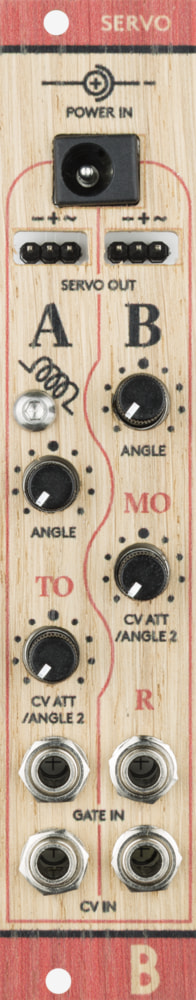
\includegraphics[width=0.75\linewidth,height=0.25\textheight,keepaspectratio]{images/bastl-servo.jpg}
  \caption{Bastl Instruments, Servo module, retrieved from their website}
  \label{fig:bastl-servo}
\end{figure}

Another inspiration came from their microgranny 2 granular sampler which is made with an Atmega microcontroller and its firmware is open source and available as a repository on their GitHub account, along with many other of their instruments.

\begin{figure}[h]
  \centering
  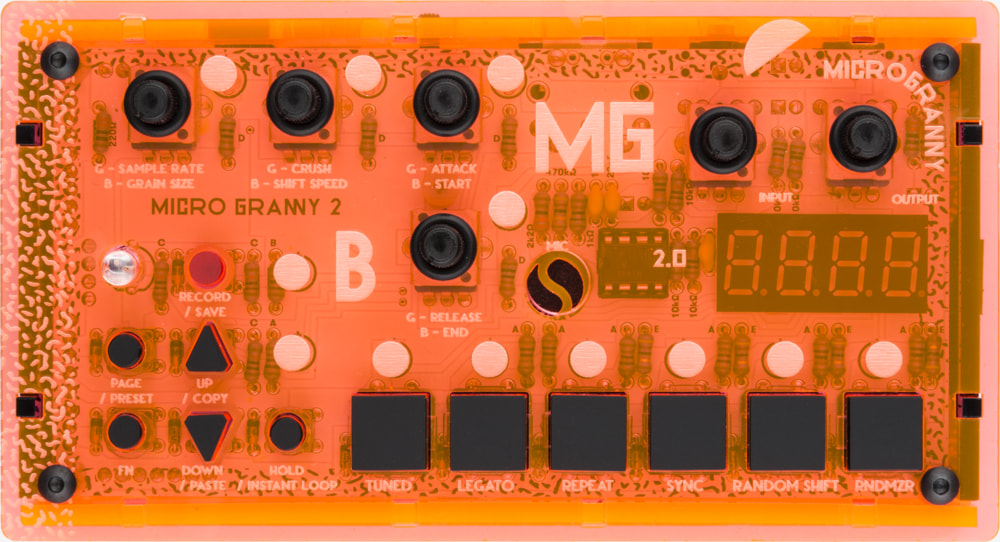
\includegraphics[width=0.75\linewidth,height=0.25\textheight,keepaspectratio]{images/bastl-microgranny-2.jpg}
  \caption{Bastl Instruments, microGranny 2, retrieved from their website}
  \label{fig:bastl-microgranny-2}
\end{figure}

Their Kastle line of synthesizers is is also based on microcontrollers, and it features a patchbay for making conections with jumper wires, the same used for prototyping in electronic breadboards, which made me lose the imposter syndrome of thinking that if I release Tiny Trainable Instruments are also valid, despite living in breadboards instead of custom printed circuit boards. Also, these are forgiving instruments, its inputs and outputs are robust enough to allow for mistakes in connections, in an electrical and mechanical way.

\begin{figure}[h]
  \centering
  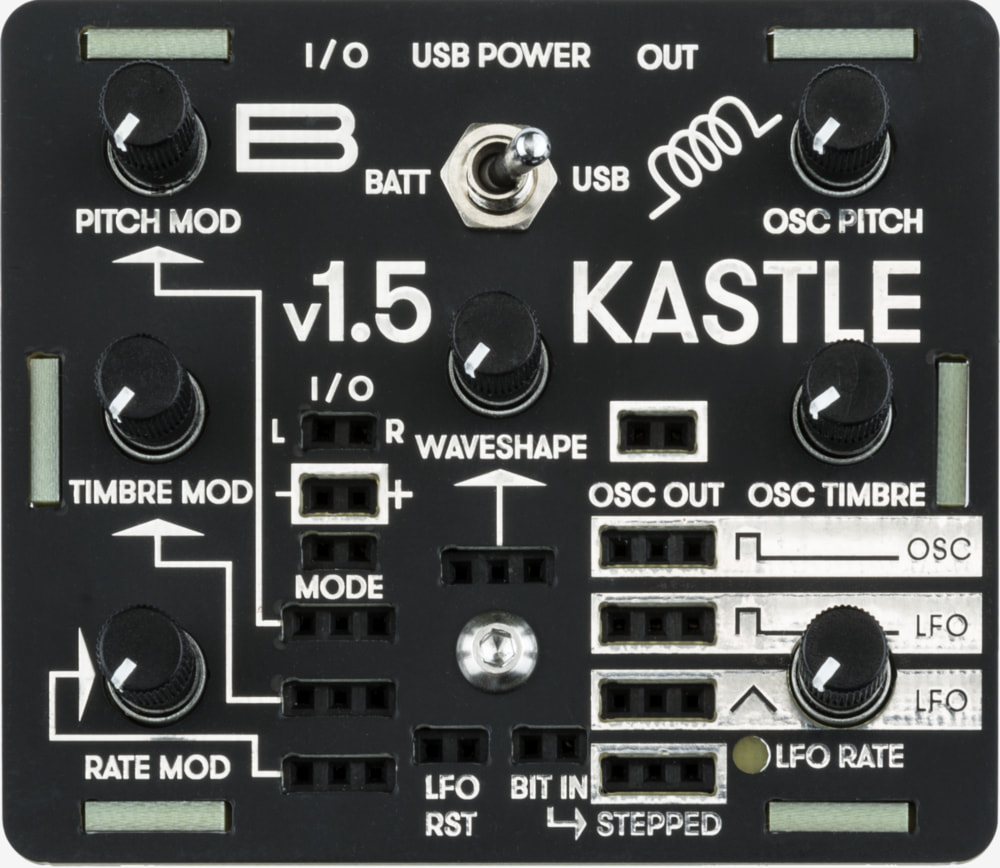
\includegraphics[width=0.75\linewidth,height=0.25\textheight,keepaspectratio]{images/bastl-kastle-v15.jpg}
  \caption{Bastl Instruments, Kastle v1.5, retrieved from their website}
  \label{fig:bastl-kastle-v15}
\end{figure}

As of writing, two different units are in production, both retailing for ~100.00 USD, the Kastle v1.5 melodic / drone synthesizer, and the Kastle Drum, for rhythm. The only difference between these synthesizers is the firmware and the labels on the faceplate. The community is encouraged to write new firmware to modify their behavior. 

\begin{figure}[h]
  \centering
  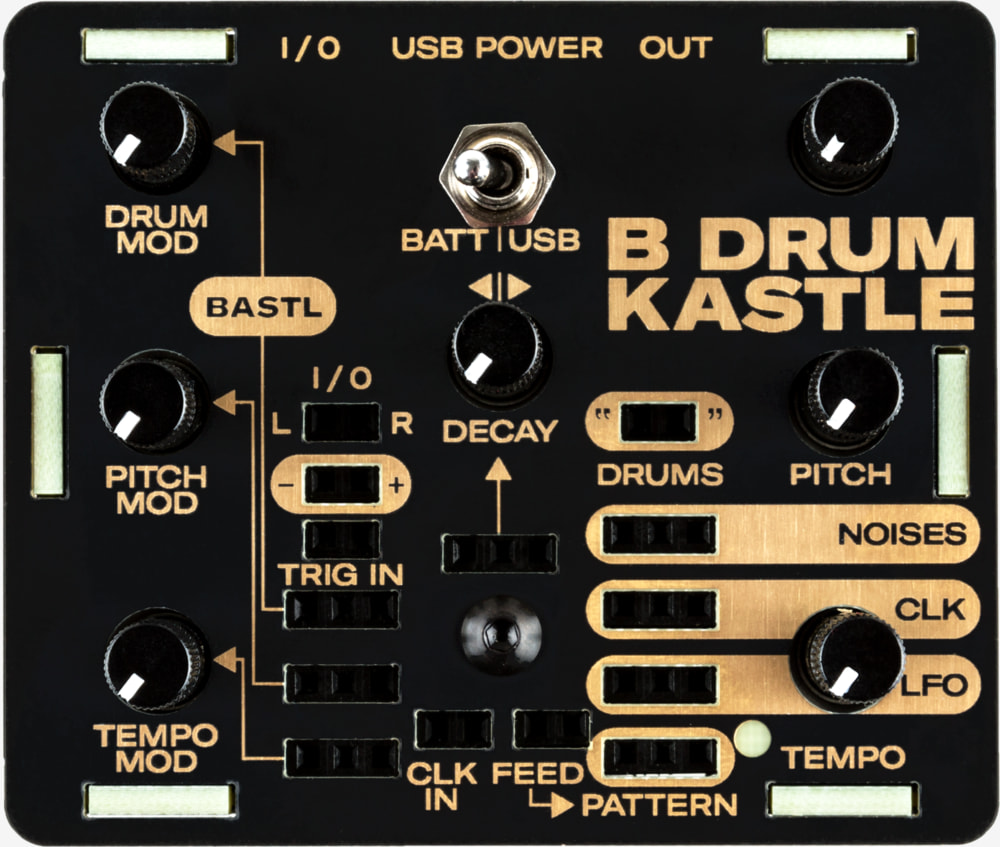
\includegraphics[width=0.75\linewidth,height=0.25\textheight,keepaspectratio]{images/bastl-kastle-drum.jpg}
  \caption{Bastl Instruments, Kastle Drum, retrieved from their website}
  \label{fig:bastl-kastle-drum}
\end{figure}

Another instrument I want to highlight is the Illuminati, currently discontinued, a device that uses different inputs (audio, control votage, MIDI messages), to control the light intensity of connected USB lamps, which influenced the conception of Tiny Trainable Instruments as multimedia arts instruments, not only focusing on audio and music.

\begin{figure}[h]
  \centering
  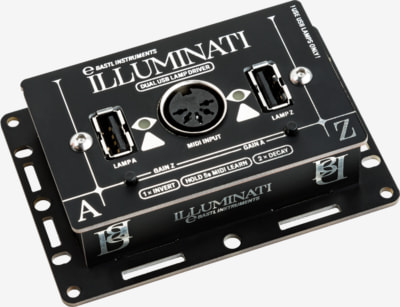
\includegraphics[width=0.75\linewidth,height=0.25\textheight,keepaspectratio]{images/bastl-illuminati.jpg}
  \caption{Bastl Instruments, Illuminati, retrieved from their website}
  \label{fig:bastl-illuminati}
\end{figure}

The final instrument from this company that I will feature is the OMSynth, one of many collaborations between Bastl and Casper Electronics. This device is an educational and maker circuit development tool for creating synthesizers, it includes basic fundamental blocks, such as battery power, audio input and output, potentiometers for attenuating and boosting signals, and a suite of parts kits for building devices including sequencers, oscillators, and samplers, on the included breadboard.

\begin{figure}[h]
  \centering
  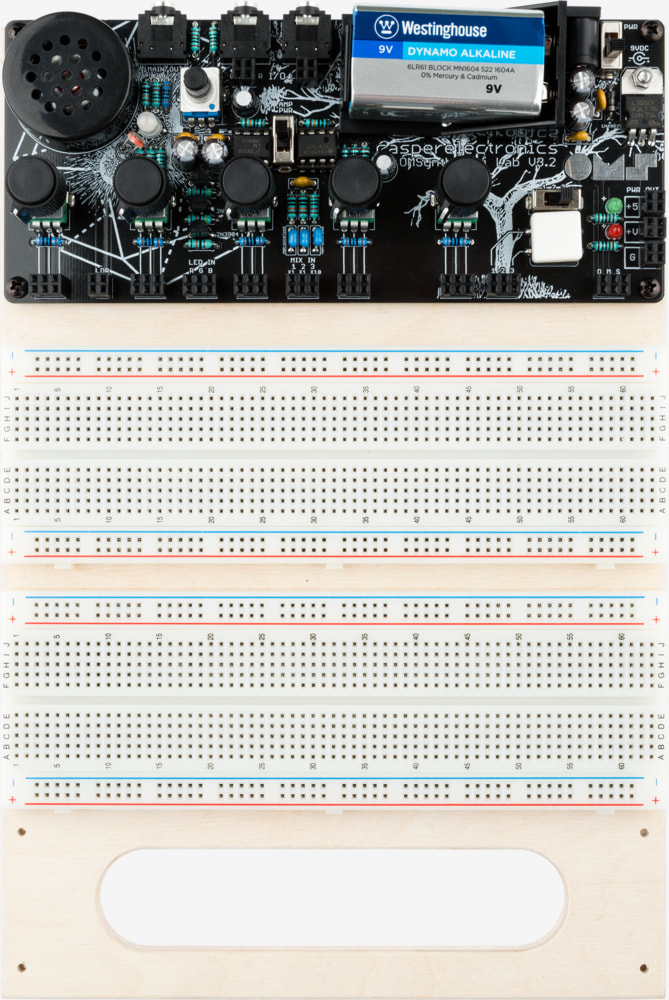
\includegraphics[width=0.75\linewidth,height=0.25\textheight,keepaspectratio]{images/bastl-omsynth.jpg}
  \caption{Bastl Instruments, OMSynth, retrieved from their website}
  \label{fig:bastl-omsynth}
\end{figure}

Many of BASTL standalone instruments are 200 USD or less, wich is a huge contrast to the 1960s, when a Moog analog system II costed 6,200 USD, which was enough to buy a small house \cite{analog-days}.

TODO: Mention how accessible the different components of the instruments are, how you can get everything from adafruit for not that much money, etc.

TODO: Add explanation about how this is not just on GitHub, but also published on the arduino IDE library, and how examples are worked already, and how things are precompiled.

TODO: Lower barriers include releasing a Bill of Materials, on Adafruit, inspired by the Drawdio project, which can be bought as a kit from Adafruit. TODO: explain why Adafruit is cool and easier to use than Digikey etc.

\subsection{Critter \& Guitari}

This company has released standalone scriptable computers for arts, which run Linux operating system + Pure Data software.

\begin{figure}[h]
  \centering
  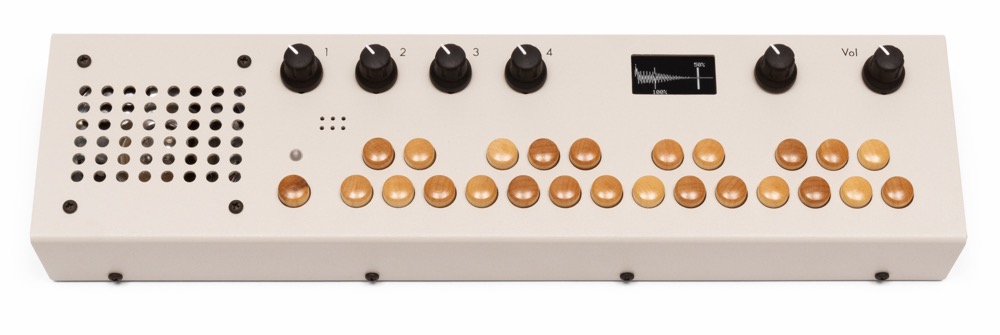
\includegraphics[width=0.75\linewidth,height=0.25\textheight,keepaspectratio]{images/critter-and-guitari-organelle-m.jpg}
  \caption{Critter \& Guitari, Organelle M, retrieved from their website}
  \label{fig:critter-and-guitari-organelle-m}
\end{figure}

ETC and EYESY computers for visuals, scriptable, Linux operating system + Python / pygame environment or openFrameworks.


\begin{figure}[h]
  \centering
  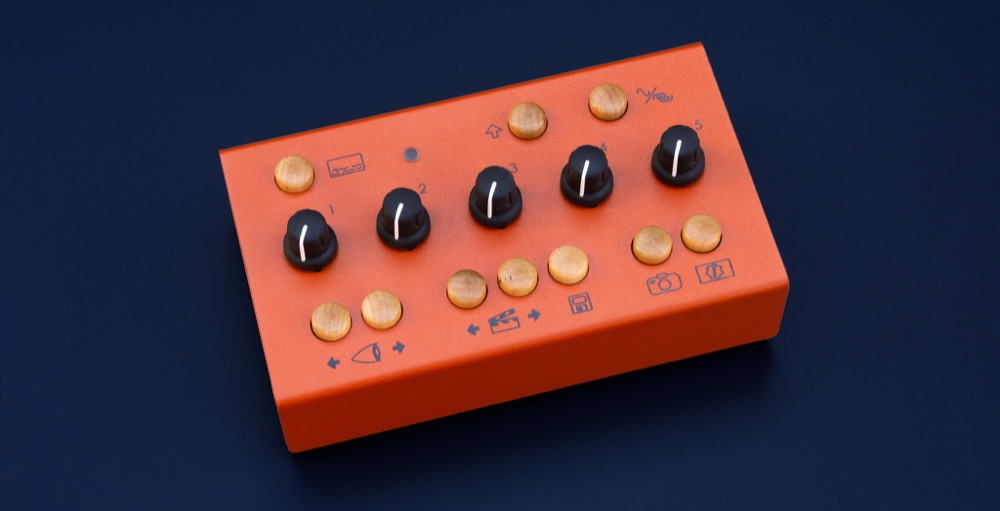
\includegraphics[width=0.75\linewidth,height=0.25\textheight,keepaspectratio]{images/critter-and-guitari-eyesy.jpg}
  \caption{Critter \& Guitari, EYESY, retrieved from their website}
  \label{fig:critter-and-guitari-eyesy}
\end{figure}

They can run on power supplies, and are also portable by the use of batteries.

\subsection{monome}

Aleph: earlier sound computer.

Norns: sound computer, currently on its second iteration, with expanded hard drive. Also there is a DIY version which is cheaper and runs on a Raspberry Pi.

Norns is a Linux machine, running SuperCollider for the sound engine, and Lua scripts. It has spawned a community that continually releases new scripts and software updates.

\subsection{Shbobo}

Peter Blasser has released several collections / companies of musical instruments, the most famous one being Ciat-Lonbarde. Peter also runs Shbobo, which to date has two different instruments, the Shnth and the Shtar.

Both run on microcontrollers, and they use a new proposed language called Shlisp, based on Lisp, and also they can be programmed using the Fish IDE.

As of 2021, they became open source, which is available at github.com/pblasser/shbobo.

COMMENT ON OPEN SOURCE: something being open source doesn't necessarily mean it is accessible to a wider audience. is one of the goals of your work to create instruments that are accessible to a wider audience?

They promote computer-centric approaches to making sound, such as the use of integers and metaphors of finite state machines, and also allow for different ways of playing and sensing, such as the use of antennas for detecting hand distance, a microphone for detecting speech and whistling, and wooden bars with piezos for detecting pressure.

TODO: write how this inspired the new interactions i am inventing or appropiating for Tiny Trainable Instruments, such as a drum machine you can talk to, Alexa spinoff.

\section{Education}

This thesis is inspired by the work of the research group Lifelong Kindergarten at MIT Media Lab, led by professor Mitchel Resnick. On the book with the same title, he builds on Seymour Papert’s work, and proposes that educational projects should have “Low floor, wide walls, high ceilings”, and that learners thrive when they engage in the 4 Ps: “Peers, projects, passion, play”
TODO: add how this project addresses the 4Ps

\section{Creative Machine learning}

COMMENT: what is the main argument of the whole piece and how does each independent part connect to that? you should start with a story from previous experiences that is particularly relevant as to why you were inspired to do this work. think "papert and the gears"

While being a graduate student and research resident at NYU ITP I saw how quick things changed in terms of machine learning. I saw how the project deeplearn.js allowed for people to train and deploy machine learning on their browsers, and how this library was acquired by Google and repurposed as TensorFlow.js, a JavaScript version of their machine learning framework TensorFlow.

In turn, at NYU ITP a team of artists and programmers built the library and community of ml5.js, with the 5 being an homage to p5.js. Technically, ml5.js is a wrapper for TensorFlow.js, in the same spirit that p5.js is a wrapper for HTML5 elements such as the canvas.

Another huge contribution to the landscape of machine learning for arts has been the release of the app Runway, which started as Cristóbal Valenzuela’s thesis, and is now a company with Alejandro Matamala and Anastasis Germanidis.

After leaving NYU ITP, I was a student at the month-long workshop “Autonomous Generative Spirit” taught by Gene Kogan and Andreas Refsgaard at the School of Machines, Make and Make Believe in Berlin 2018. We experimented with quick and cheap methods for machine learning, such as the k-nearest neighbors algorithm using the artist and beginner-friendly app Wekinator by Rebecca Fiebrink, and also more computer-intensive algorithms, which sometimes required proprietary hardware such as NVIDIA graphics cards to be trained in a matter of hours, instead of days or weeks using our computers.

TODO: add what does the speed enable you to do on a personal level? why is it important to share that speed with others?

The last spark that led me to this thesis was the release of two libraries for machine learning on the Arduino platform: The currently beta version Arduino KNN, which allows for on-device training and resembles my earlier studies with Wekinator, in a more portable and private way, no data leaves the microcontroller, and the whole neural network can be wiped with one click of a button.

At a more complex level, I am also working with the TensorFlow Lite Micro, which I learned from Arduino blogs, and which currently is supported by the hardware Arduino Nano 33 BLE Sense.

COMMENT TO THE ABOVE PARAGRAPH: you may not even need to include the specific details here, but just highlight in larger overviews the types of projects you've worked on or the educational fields that influence your work

In late 2020 and early 2021 I completed the just released series of 3 courses of the TinyML Professional Certificate by Harvard at the online platform edx.org

Newer books and references that this thesis was inspired by include the books “You Look Like a Thing and I Love You: How Artificial Intelligence Works and Why It's Making the World a Weirder Place” by Janelle Shane (2019), and the book “Making Pictures with Generative Adversarial Networks” by Casey Reas (2019).

Also Yining Shi created a new class at NYU ITP in 2020, at the intersection of machine learning and physical computing.

\section{Digital rights}

Machine learning algorithms need data to be trained on. I think it’s a human right to not be surveilled, and I hope my thesis can put a positive spin on the gathering of data, by letting users perform auto surveillance, like the Ai Weiwei piece WeiweiCam, a 2021 project where the artist installed cameras for self surveillance as a protest against the Chinese government.

A huge inspiration for my thesis has been the Guardian Project by the Electronic Frontier Foundation, and the Design Justice Network and the book Design Justice by Sasha Costanza-Chock.

TODO QUESTION: is any of the methodology you use to develop all of this work specifically related to either of these? you might connect specific aspects of the EFF project and Sasha's work that are connected


\section{Instruments}

The table \ref{table:media-arts-scriptable-instruments} is an example of media arts instruments that are scriptable.

\begin{table}[h!]
    \centering
    \begin{tabular}{ | l | l | l | l | l | }
        Maker & Instrument & Year & Computing & Software \\ 
        \hline 
        BASTL & microGranny 2 & YEAR & microcontroller & Arduino \\
        BASTL & Kastle v1.5 & YEAR &microcontroller  & Arduino \\
        Critter \& Guitari & Organelle & YEAR & computer & Linux? \\
        Critter \& Guitari & EYESY & YEAR & computer & Linux? \\
        monome & aleph & YEAR & computer & Linux? \\
        monome & norns & YEAR & computer & Linux \\
        Shbobo & Shnth & YEAR & microcontroller & ARM Cortex \\
        Shbobo & Shtar & YEAR & microcontroller & ARM Cortex 
    \end{tabular}
    \caption{Table of media arts scriptable instruments}
    \label{table:media-arts-scriptable-instruments}
\end{table}


\subsection{BASTL}

BASTL Kastle, two iterations and a spinoff: Kastle, Kastle v1.5, Kastle Drum. 

Based on Arduino, GitHub repository with alternate firmware.

Breadboard patching with jumper cables, inputs and outputs robust enough to allow for mistakes in connections.

\subsection{Critter \& Guitari}

Organelle computer for sound, scriptable, Linux operating system + Pure Data software.

ETC and EYESY computers for visuals, scriptable, Linux operating system + Python / pygame environment or openFrameworks.

\subsection{monome}

Aleph: sound computer

Norns: sound computer, currently on its second iteration, with expanded hard drive. Also there is a DIY versionm which is cheaper and runs on a Raspberry Pi.
Norns is a Linux machine, running SuperCollider for the sound engine, and Lua scripts.

\subsection{Shbobo}

Peter Blasser's Shbobo

Shnth and Shtar

Shlisp language and Fish IDE.

github.com/pblasser/shbobo

\section{Education}

Mitch Resnick's book Lifelong Kindergarten

Low floor, wide walls, high ceiling

Peers, projects, passion, play

Gene Kogan and Andreas Refsgaard

\section{Machine learning}

ml5.js

Runway

TinyML Professional Certificate HarvardX

\section{Digital rights}

Electronic Frontier Foundation

Edward Snowden

Design Justice Network
